\documentclass[11pt,a4paper]{article}

\usepackage[T1]{fontenc}
\usepackage[utf8]{inputenc}
\usepackage[brazilian]{babel}
\usepackage[margin=2.5cm]{geometry}
\usepackage{graphicx}
\usepackage{booktabs}
\usepackage{amsmath}
\usepackage[hidelinks]{hyperref}

\graphicspath{{../figures/}}

\setlength{\parskip}{0.5em}
\setlength{\parindent}{0pt}

\title{\textbf{Modelo SIR para uma epidemia de chikungunya no Recife}}
\author{Leandro Cesar}
\date{Elementos de Epidemiologia Computacional \\ BSI UFRPE \\[0.6em] Setembro de 2026}

\begin{document}

\maketitle

\begin{abstract}
\noindent
Este trabalho aplica o modelo SIR clássico à introdução do vírus chikungunya no município do Recife.
A doença foi escolhida por três razões: a imunidade após a infecção é duradoura, a população era
imunologicamente virgem quando o vírus chegou à cidade em 2015, e o surto se concentra em uma única onda.
Com $N = 1.488.920$ habitantes, período infeccioso de 7 dias e $R_0 = 3{,}4$ retirado de revisão
sistemática, o modelo prevê pico no dia 44 com 514.377 pessoas infectadas simultaneamente, 34,5 por cento
da população. Oito variações das taxas de contágio e de recuperação mostram que a razão entre elas fixa
o tamanho da epidemia enquanto a escala fixa apenas a sua velocidade. A discussão final confronta a taxa
de ataque prevista, de 96,2 por cento, com a soroprevalência de 11,8 por cento medida em inquérito de
campo no Nordeste, e usa essa distância para dimensionar o custo da hipótese de mistura homogênea.
\end{abstract}

\section{A doença escolhida}

O vírus chikungunya foi introduzido no Brasil em 2014 e chegou ao Recife em meados de 2015. O estudo de
vigilância conduzido no município detectou os primeiros casos em junho de 2015 e um crescimento acentuado
a partir de agosto, ao ponto de a circulação do chikungunya deslocar a do zika na cidade
\cite{magalhaes2017}.

Três características tornam a chikungunya um objeto adequado para um modelo SIR.

A primeira é que a imunidade após a infecção é duradoura. A Organização Mundial da Saúde indica que quem
se recupera provavelmente fica imune a infecções futuras \cite{who}, o que justifica um compartimento $R$
absorvente, sem retorno para $S$.

A segunda é que a população era imunologicamente virgem. Como o vírus nunca havia circulado no Recife
antes de 2015, a condição inicial adotada no curso, com toda a população em $S$ e um único caso em $I$,
deixa de ser uma idealização didática e passa a descrever o cenário real de introdução.

A terceira é que o surto é único e concentrado no tempo, o que dispensa a modelagem de reintroduções
sazonais repetidas para descrever a primeira onda.

A simplificação central, retomada na seção \ref{sec:lacunas}, é que o mosquito \textit{Aedes aegypti} não
aparece no modelo. A transmissão de pessoa para pessoa é tratada como direta e o vetor fica implícito
dentro da taxa de contágio.

\section{O modelo}

A população de tamanho $N$ é dividida em suscetíveis $S$, infectados $I$ e recuperados $R$, na formulação
de Kermack e McKendrick \cite{kermack1927}. A força de infecção é dinâmica, isto é, proporcional à fração
da população infectada no instante considerado:

\begin{equation}
\lambda = \beta \frac{I}{N}
\end{equation}

\begin{equation}
\frac{dS}{dt} = -\lambda S, \quad
\frac{dI}{dt} = \lambda S - \gamma I, \quad
\frac{dR}{dt} = \gamma I
\end{equation}

O número básico de reprodução é a razão entre as duas taxas, $R_0 = \beta / \gamma$. A figura
\ref{fig:diagrama} apresenta a estrutura de compartimentos com os valores adotados.

\begin{figure}[!ht]
\centering
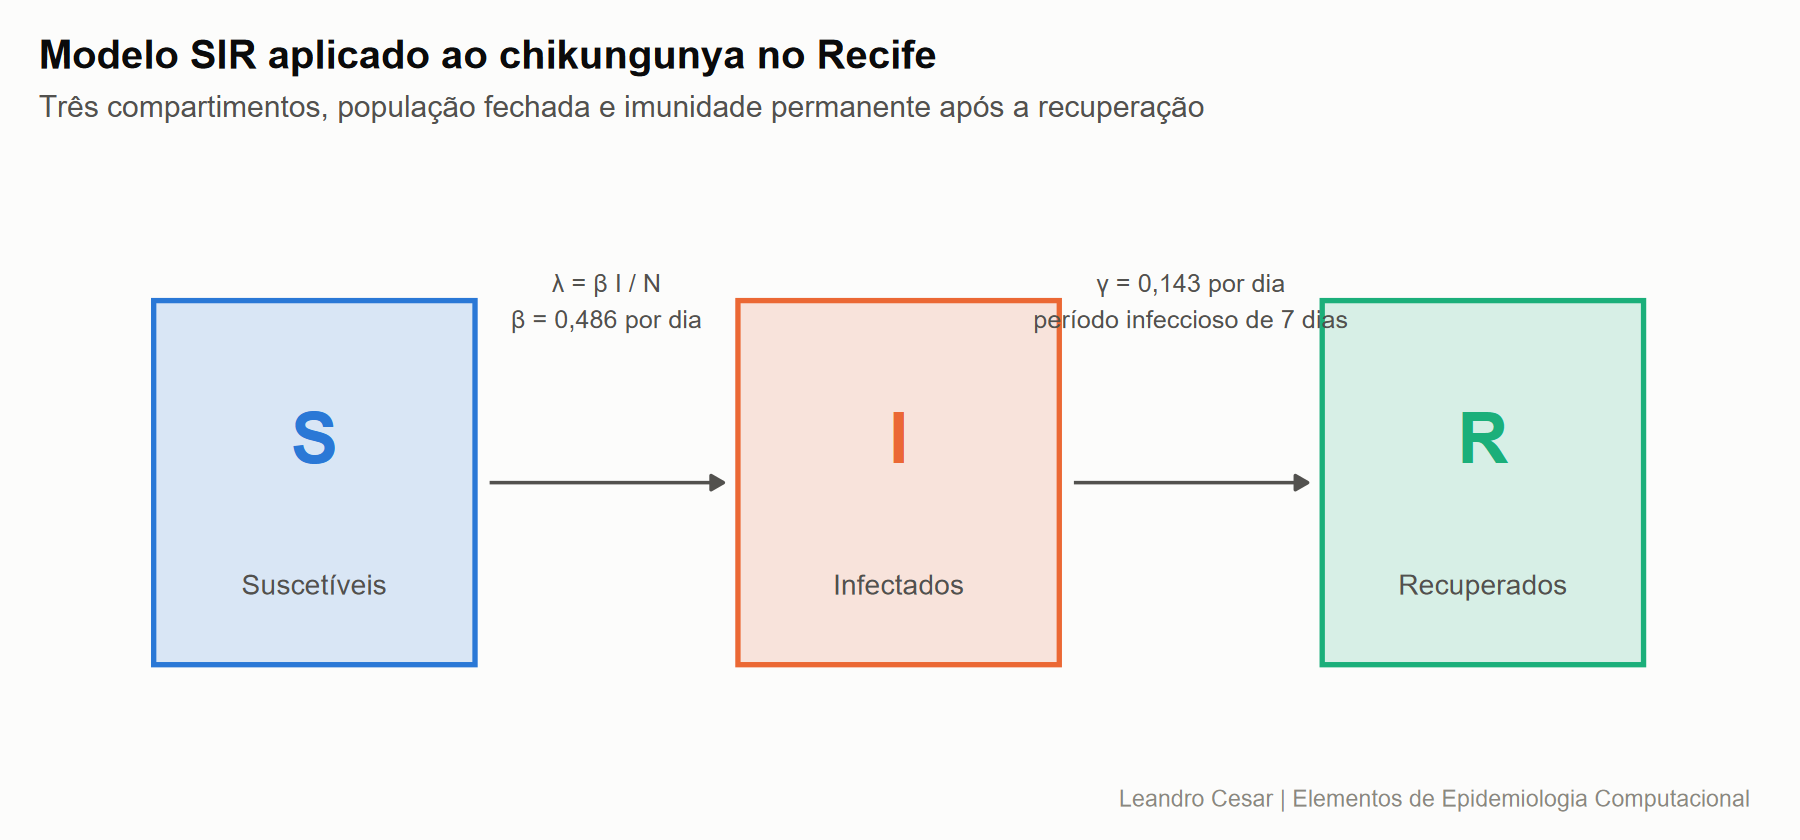
\includegraphics[width=\textwidth]{fig1_diagrama_sir.png}
\caption{Estrutura de compartimentos do modelo SIR com os parâmetros do estudo.}
\label{fig:diagrama}
\end{figure}

As hipóteses assumidas são a homogeneidade da população dentro de cada compartimento, a mistura homogênea
entre suscetíveis e infectados, a população fechada com $S + I + R = N$ constante, a imunidade permanente,
a infecciosidade imediata sem período de latência, e taxas constantes ao longo de todo o surto.

\section{Parâmetros e justificativa}

A tabela \ref{tab:parametros} reúne os valores adotados. Nenhum deles foi arbitrado sem referência.

\begin{table}[!ht]
\centering
\caption{Parâmetros do modelo e suas justificativas.}
\label{tab:parametros}
\small
\begin{tabular}{lll}
\toprule
\textbf{Parâmetro} & \textbf{Valor} & \textbf{Origem} \\
\midrule
$N$ & 1.488.920 & Censo 2022 do IBGE \cite{ibge2022} \\
$S_0$ & $N - 1$ & Sem imunidade prévia \\
$I_0$ & 1 & Caso introduzido \\
$R_0$ inicial & 0 & Nenhum recuperado \\
$\gamma$ & $1/7$ por dia & Viremia de 5 a 7 dias \cite{cdc} \\
$R_0$ & 3,4 & Revisão sistemática \cite{liu2020} \\
$\beta$ & 0,486 por dia & Derivado de $R_0 \gamma$ \\
Horizonte & 180 dias & Cobre o surto completo \\
\bottomrule
\end{tabular}
\end{table}

Duas escolhas merecem destaque.

A primeira é $\gamma$. Ele é definido a partir da viremia humana, que é o intervalo em que a pessoa pode
infectar um mosquito. Como o modelo não representa o vetor, o intervalo entre duas infecções humanas
consecutivas fica menor do que o intervalo serial real do chikungunya, que inclui a incubação extrínseca
no mosquito. O efeito prático é que a epidemia simulada corre mais rápido do que a observada. O cenário 7
da seção \ref{sec:variacoes} quantifica esse efeito.

A segunda é $\beta$. Em vez de escolher uma taxa de contágio diretamente, ela é obtida de $R_0$, que é a
grandeza efetivamente estimada em campo. A revisão sistemática de Liu e colaboradores reporta média
ponderada de 3,4, com intervalo de confiança de 95 por cento entre 2,4 e 4,2, e valor de 4,1 quando o
vetor é o \textit{Aedes aegypti} \cite{liu2020}. Adotou-se a média ponderada geral, que é o valor mais
conservador dentro do que a literatura sustenta.

\section{O pico da epidemia}

As equações foram integradas com o pacote \texttt{deSolve} \cite{desolve}, em passo diário, ao longo de
180 dias. A figura \ref{fig:base} mostra a evolução dos três compartimentos e a figura \ref{fig:pico}
detalha o pico.

\begin{figure}[!ht]
\centering
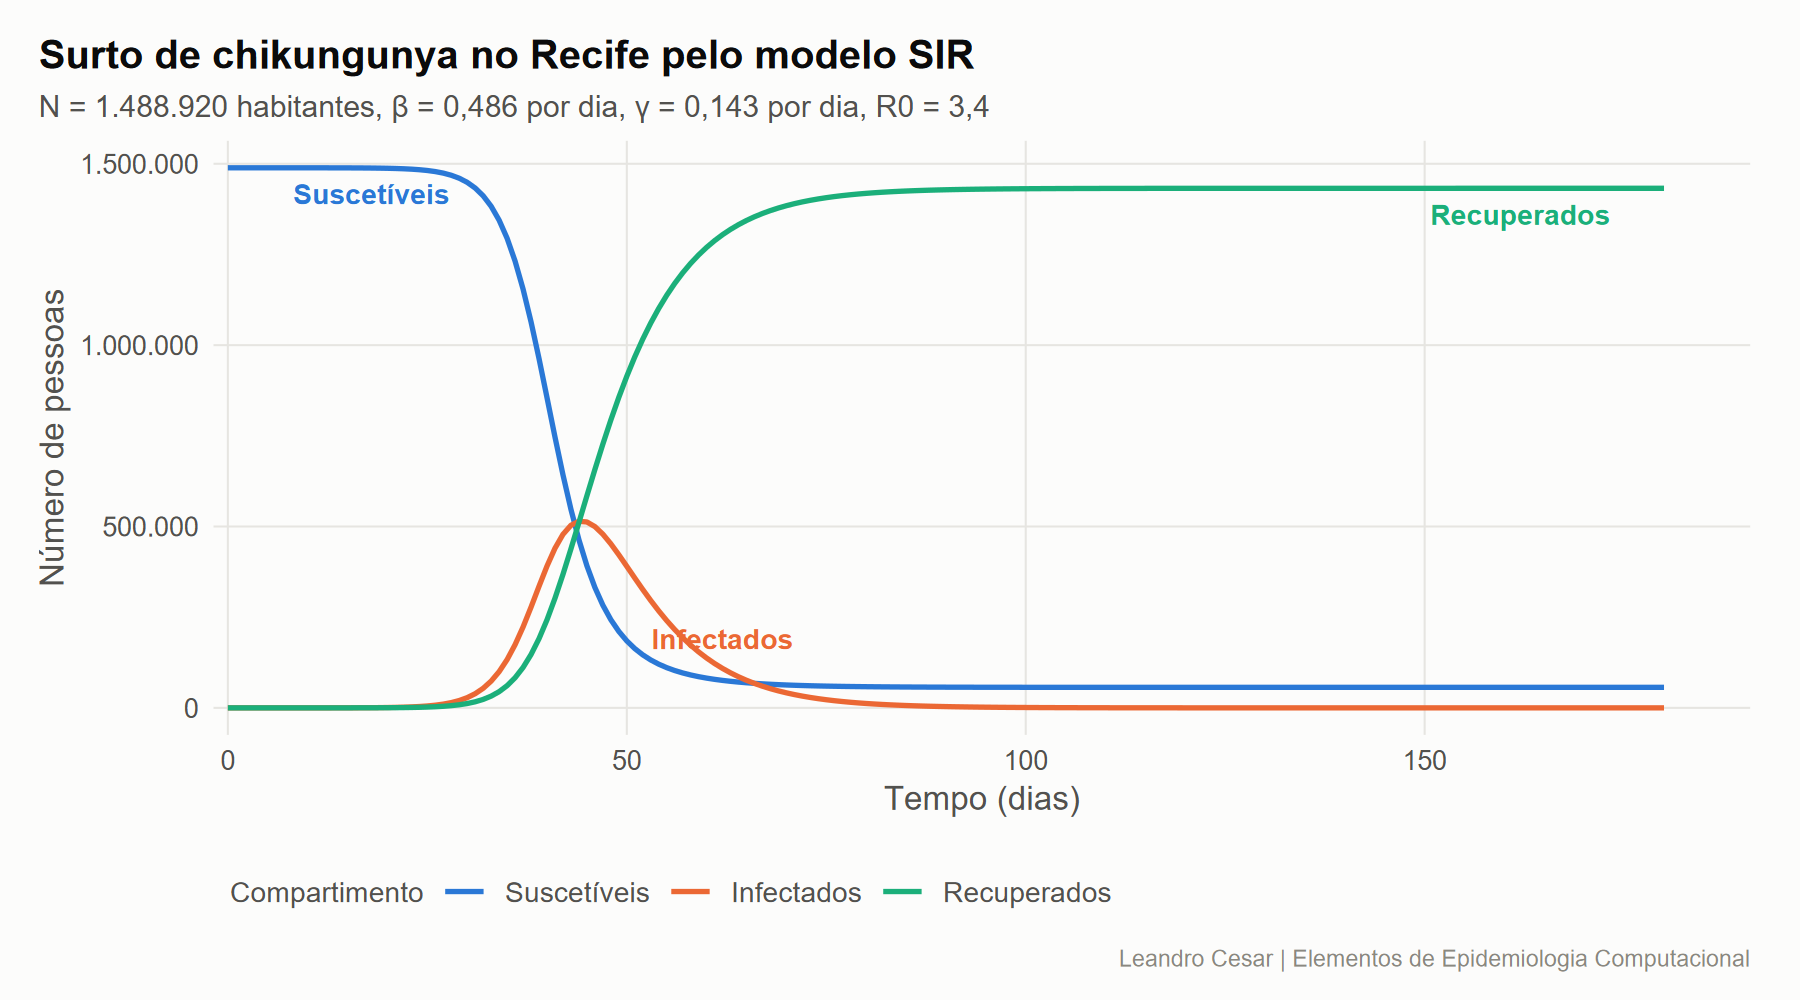
\includegraphics[width=\textwidth]{fig2_linha_base_sir.png}
\caption{Evolução dos compartimentos na linha de base.}
\label{fig:base}
\end{figure}

\begin{figure}[!ht]
\centering
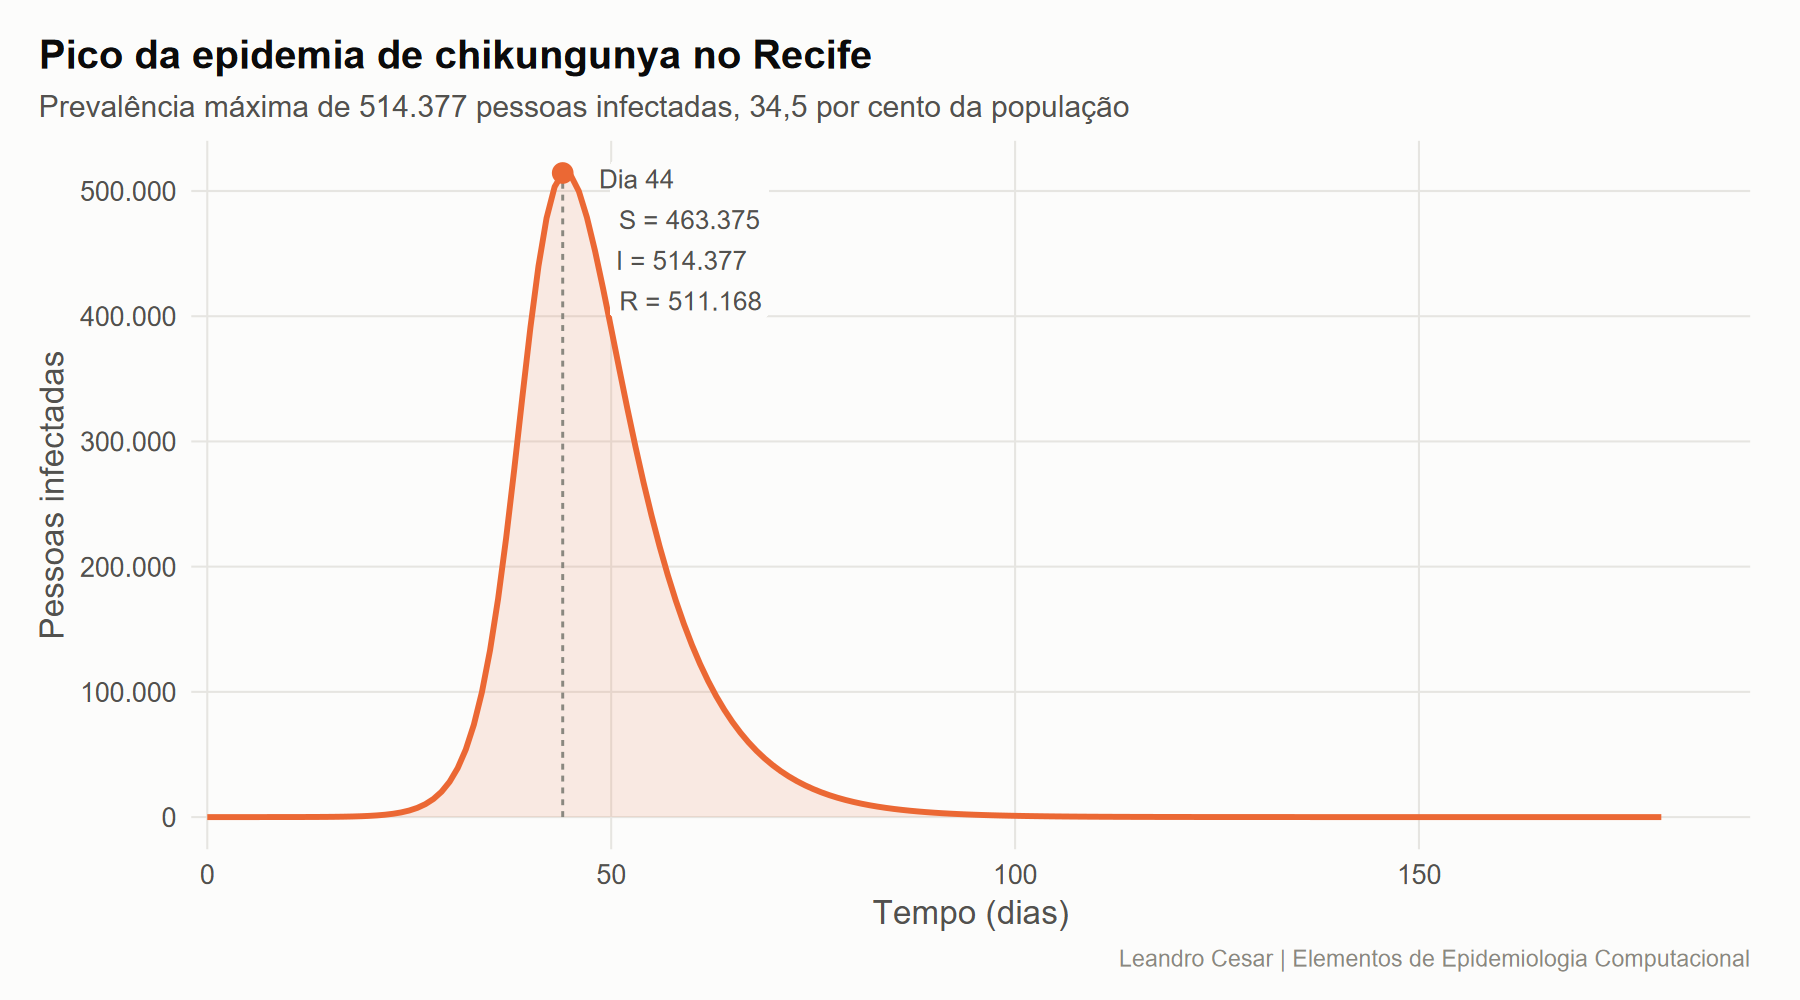
\includegraphics[width=\textwidth]{fig3_pico_epidemico.png}
\caption{Curva de infectados com o pico destacado.}
\label{fig:pico}
\end{figure}

A epidemia atinge o pico no dia 44. A tabela \ref{tab:pico} apresenta a ocupação dos compartimentos nesse
dia.

\begin{table}[!ht]
\centering
\caption{Compartimentos no dia do pico, dia 44.}
\label{tab:pico}
\begin{tabular}{lrr}
\toprule
\textbf{Compartimento} & \textbf{Pessoas} & \textbf{Fração} \\
\midrule
Suscetíveis & 463.375 & 31,1 \% \\
Infectados & 514.377 & 34,5 \% \\
Recuperados & 511.168 & 34,3 \% \\
\bottomrule
\end{tabular}
\end{table}

O resultado numérico coincide com a teoria. Refinando o passo de integração para 0,05 dia, o pico aparece
em 44,35 dias com 515.089 infectados, valor que reproduz a expressão analítica da prevalência máxima,

\begin{equation}
\frac{I_{max}}{N} = 1 - \frac{1 + \ln R_0}{R_0} = 0{,}346
\end{equation}

e o número de suscetíveis nesse instante reproduz $N / R_0 = 437.918$ pessoas. Esse é o significado
geométrico do pico: ele ocorre exatamente quando a reserva de suscetíveis cruza o limiar $N / R_0$, e não
em um instante arbitrário. A taxa de ataque final simulada, de 96,2 por cento, coincide com a raiz da
equação implícita $1 - a = e^{-R_0 a}$ com seis casas decimais.

\section{Variações nas taxas}
\label{sec:variacoes}

Foram simulados oito cenários, que cobrem as três situações sugeridas no enunciado e acrescentam duas
análises. A tabela \ref{tab:cenarios} resume os resultados e as figuras \ref{fig:painel},
\ref{fig:infectados} e \ref{fig:limiar} os apresentam graficamente.

\begin{table}[!ht]
\centering
\caption{Os oito cenários e seus desfechos.}
\label{tab:cenarios}
\footnotesize
\setlength{\tabcolsep}{4pt}
\begin{tabular}{clrrrrrr}
\toprule
\textbf{N} & \textbf{Cenário} & $\beta$ & $\gamma$ & $R_0$ & \textbf{Pico (dia)} & \textbf{Pico} & \textbf{Ataque} \\
\midrule
1 & Linha de base & 0,486 & 0,143 & 3,40 & 44 & 514.377 & 96,2 \% \\
2 & Taxas iguais & 0,143 & 0,143 & 1,00 & sem surto & sem surto & 0,0 \% \\
3 & Contágio pela metade & 0,243 & 0,143 & 1,70 & 136 & 148.295 & 69,1 \% \\
4 & Contágio 50\% maior & 0,729 & 0,143 & 5,10 & 27 & 721.315 & 99,4 \% \\
5 & Viremia de 14 dias & 0,486 & 0,071 & 6,80 & 39 & 850.233 & 99,9 \% \\
6 & Recuperação em 1,7 dia & 0,486 & 0,600 & 0,81 & sem surto & sem surto & 0,0 \% \\
7 & Mesmo $R_0$, ritmo 1/2 & 0,243 & 0,071 & 3,40 & 89 & 514.926 & 96,2 \% \\
8 & Controle vetorial do Aedes & 0,194 & 0,143 & 1,36 & 243 & 57.494 & 47,8 \% \\
\bottomrule
\end{tabular}
\end{table}

\begin{figure}[!ht]
\centering
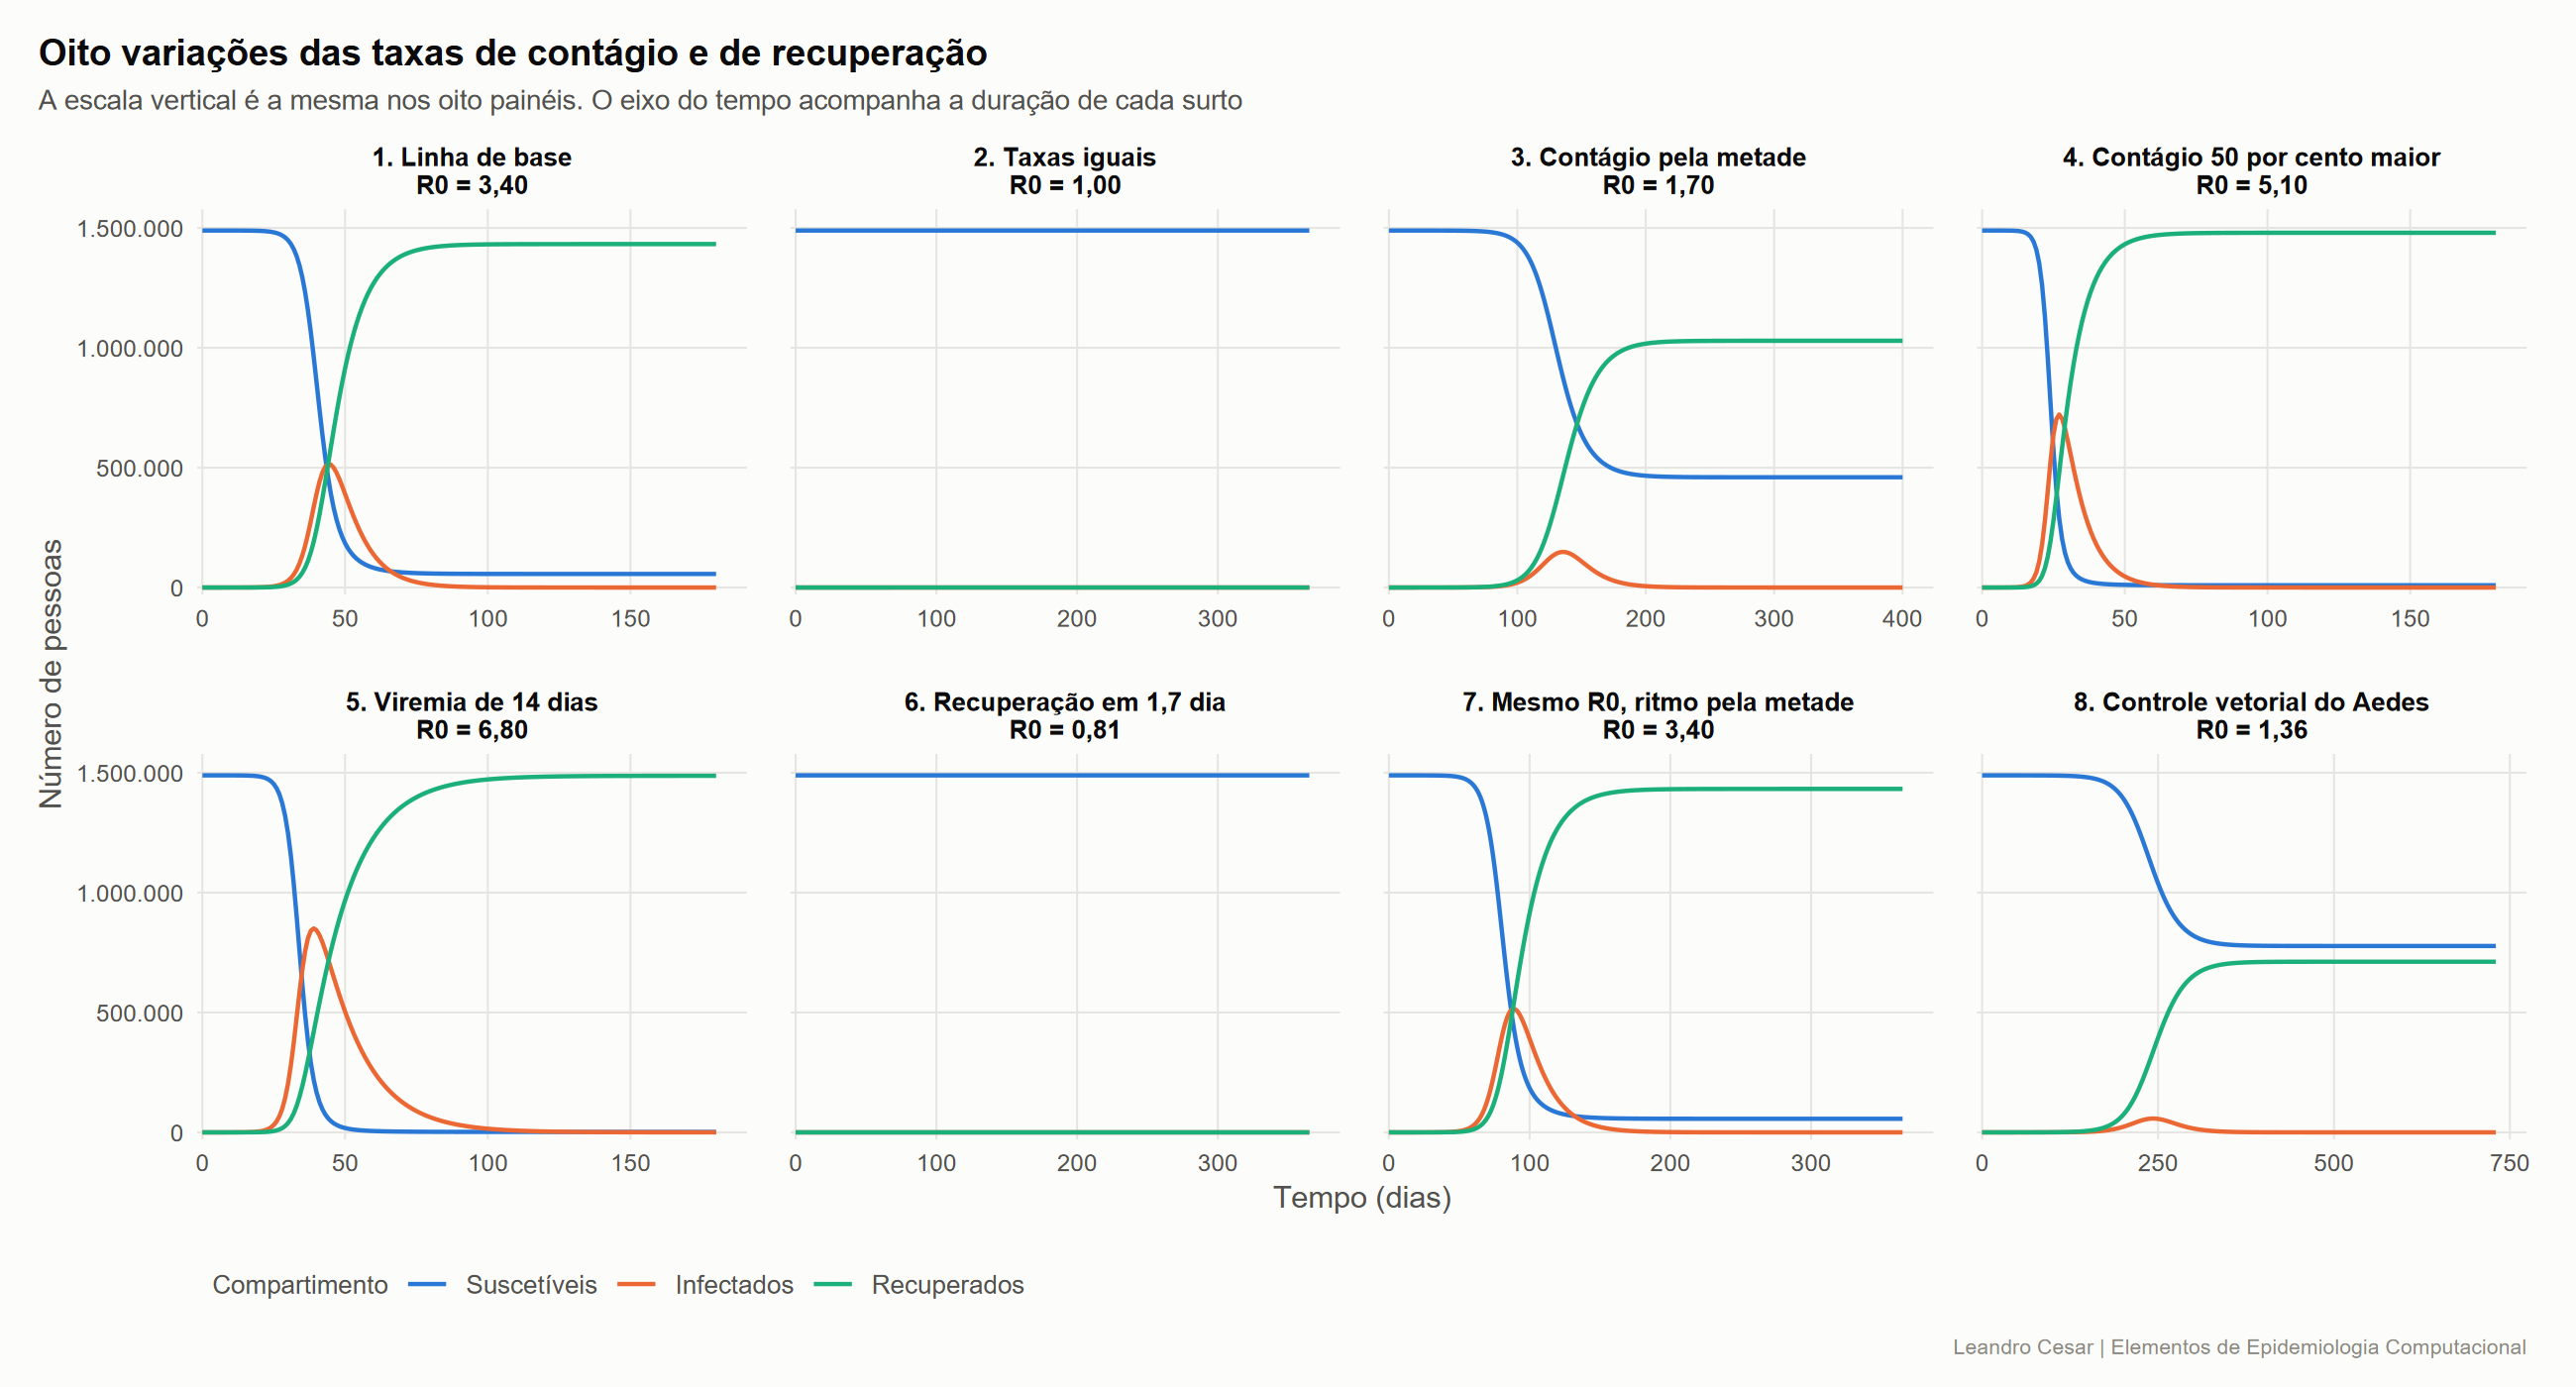
\includegraphics[width=\textwidth]{fig4_cenarios_painel.png}
\caption{Os oito cenários com os três compartimentos, em escala vertical comum.}
\label{fig:painel}
\end{figure}

\begin{figure}[!ht]
\centering
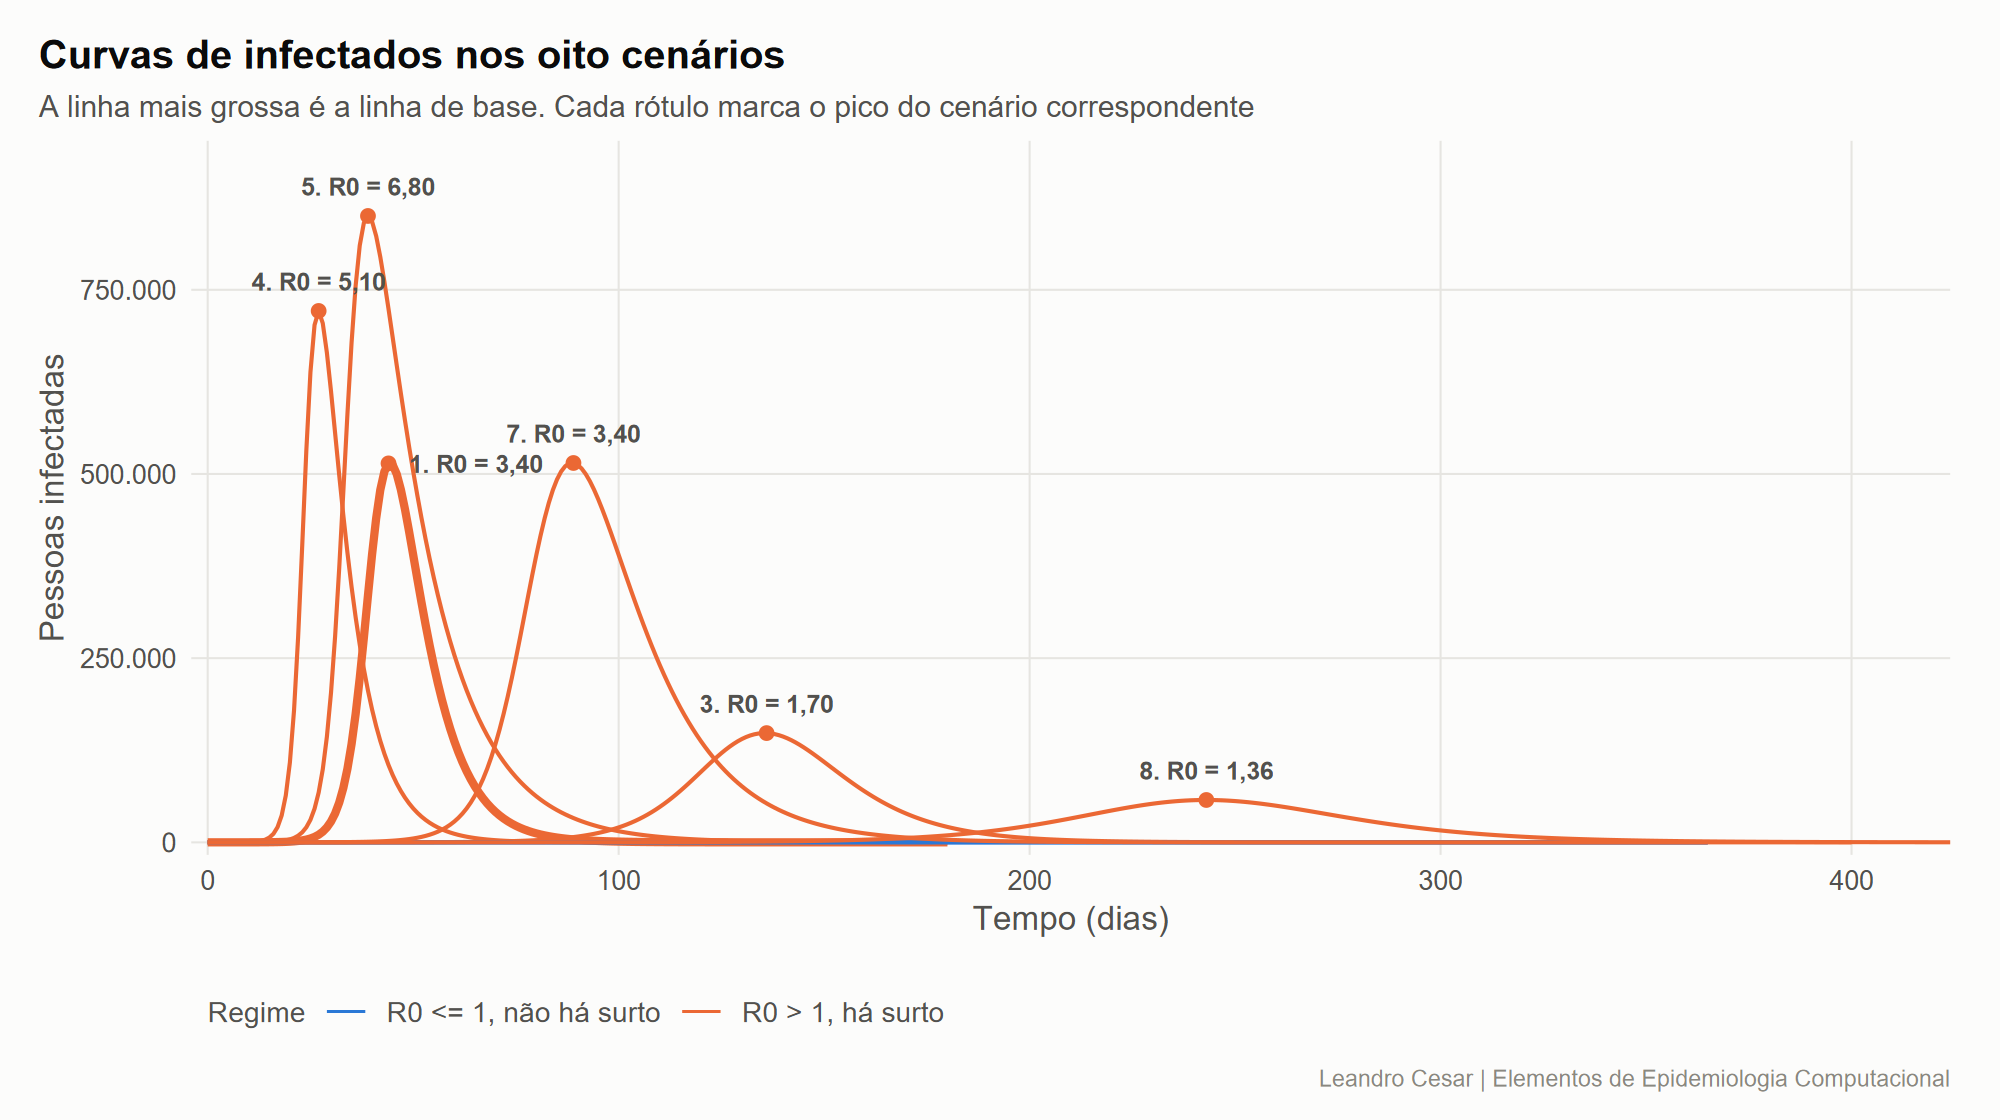
\includegraphics[width=\textwidth]{fig5_cenarios_infectados.png}
\caption{Curvas de infectados sobrepostas, com o pico de cada cenário marcado.}
\label{fig:infectados}
\end{figure}

\begin{figure}[!ht]
\centering
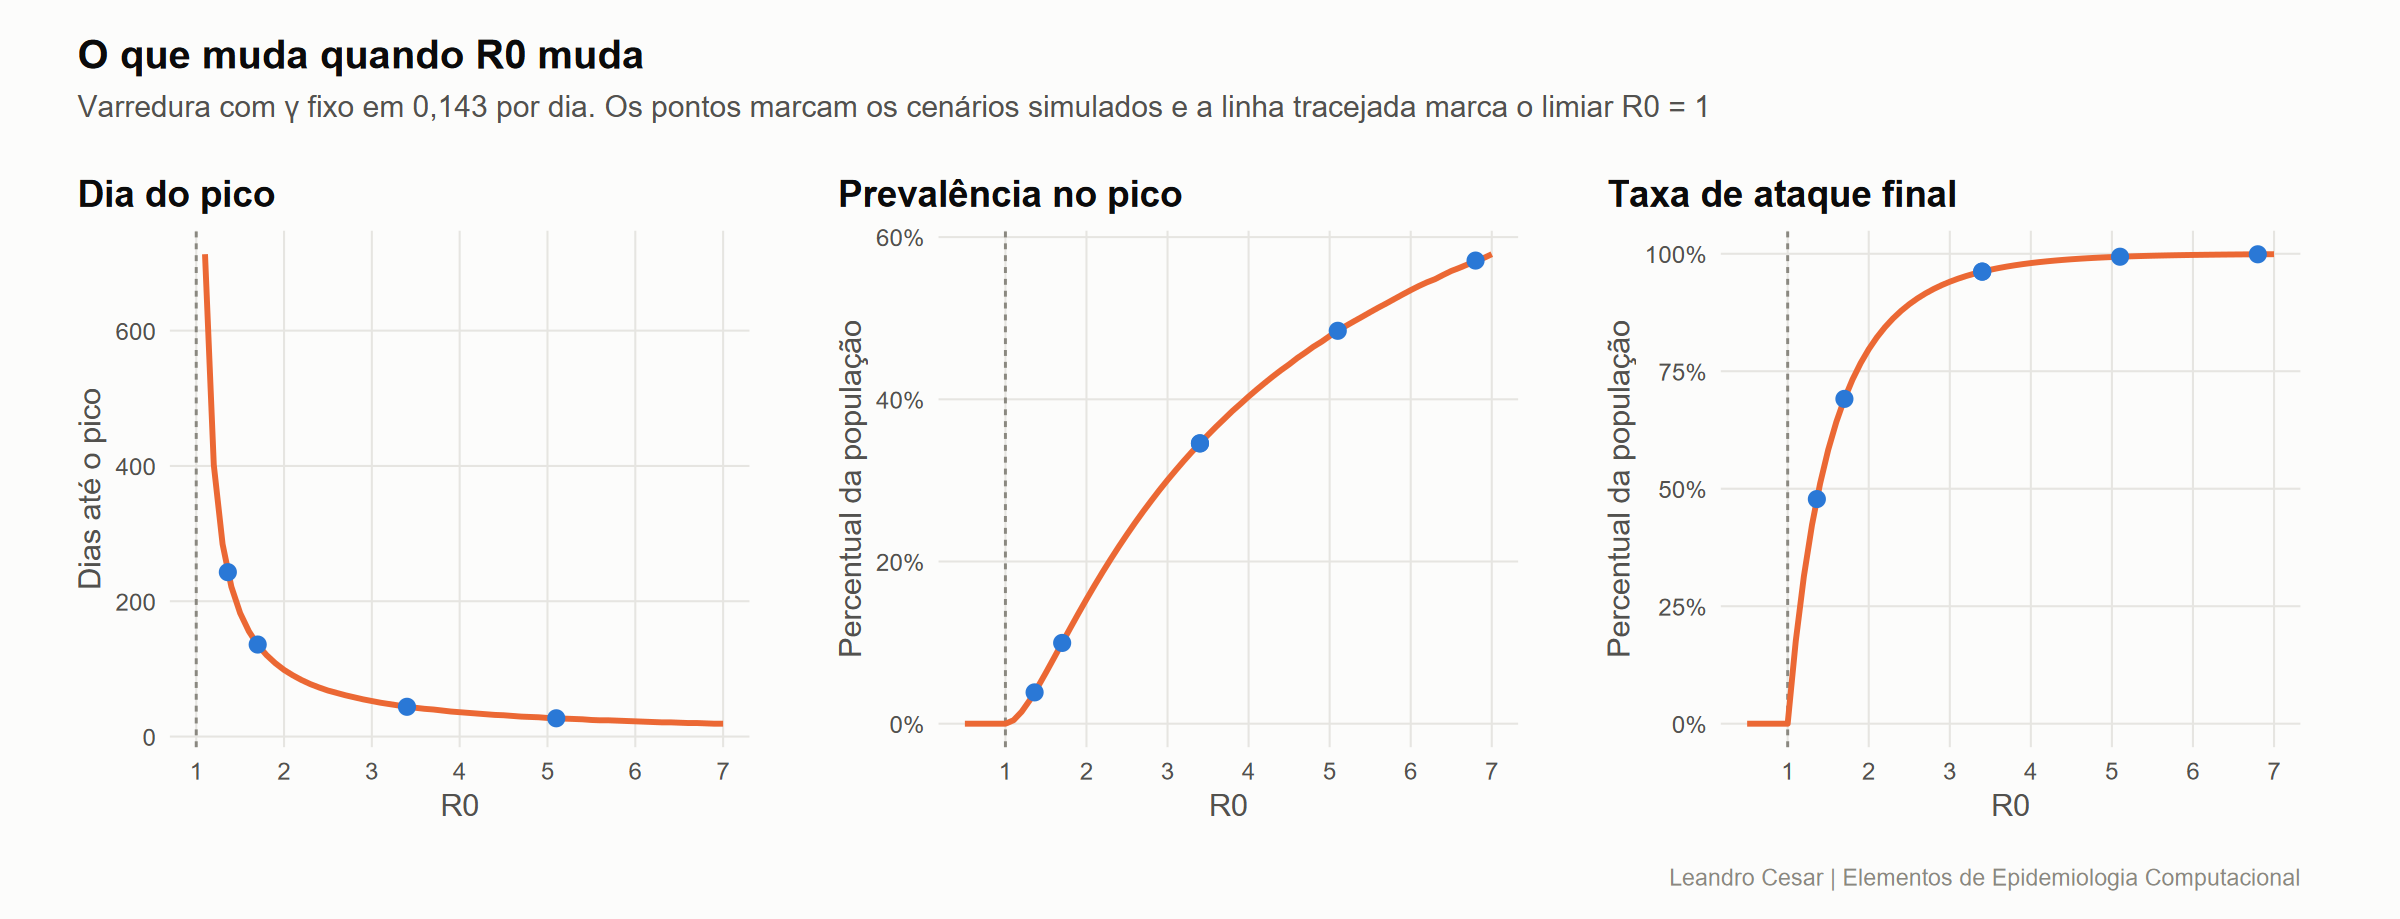
\includegraphics[width=\textwidth]{fig6_limiar_r0.png}
\caption{Dependência dos três desfechos em relação a $R_0$, com $\gamma$ mantido fixo.}
\label{fig:limiar}
\end{figure}

\textbf{Taxas iguais.} Com $\beta$ igual a $\gamma$, o valor de $R_0$ é exatamente 1 e nada acontece.
Cada infectado transmite em média para exatamente uma outra pessoa, então a prevalência não cresce nem
decai. Esse é o limiar epidêmico, e ele separa dois comportamentos qualitativamente distintos, não apenas
dois surtos de tamanhos diferentes.

\textbf{Recuperação fixa, contágio variando.} Aumentar o contágio adianta e agrava o surto. Passando de
$\beta = 0{,}243$ para $\beta = 0{,}729$, o pico salta do dia 136 para o dia 27 e sobe de 148 mil para 721
mil infectados. A curva também fica mais estreita, porque quanto mais rápido o surto sobe, mais rápido ele
esgota os suscetíveis e desce.

\textbf{Contágio fixo, recuperação variando.} A taxa de recuperação atua no sentido oposto. Dobrando o
período infeccioso de 7 para 14 dias, $R_0$ dobra para 6,8 e o pico atinge 850 mil pessoas. No outro
extremo, uma recuperação em 1,7 dia derruba $R_0$ para 0,81 e o surto não ocorre. O cenário 6 não
representa um surto pequeno, e sim a ausência de surto, assim como o cenário 2.

\textbf{Mesmo $R_0$ com ritmo pela metade.} Dividindo $\beta$ e $\gamma$ pelo mesmo fator, $R_0$ permanece
em 3,4. A altura do pico e a taxa de ataque final ficam idênticas às da linha de base, mas o pico passa do
dia 44 para o dia 89, exatamente o dobro do tempo. A razão entre as taxas determina o tamanho da epidemia
e a escala das taxas determina apenas a sua velocidade. É por isso que a subestimação do intervalo serial
apontada na seção anterior afeta o calendário do surto, mas não o número de pessoas atingidas.

\textbf{Controle vetorial.} Reduzir o contágio em 60 por cento, efeito esperado de uma campanha eficaz
contra criadouros, baixa $R_0$ para 1,36. O pico cai de 514 mil para 57 mil infectados, redução de quase
nove vezes, e é empurrado do dia 44 para o dia 243. A taxa de ataque cai de 96 para 48 por cento. Este é
o achatamento da curva no modelo mais simples possível.

\textbf{Leitura conjunta.} A figura \ref{fig:limiar} explica por que os cenários se organizam assim. A
prevalência no pico e a taxa de ataque final dependem apenas de $R_0$, e ambas crescem rápido logo acima
do limiar e depois saturam. Já o dia do pico depende também da escala das taxas, e por isso apenas os
cenários que compartilham o mesmo $\gamma$ aparecem no primeiro painel. Ganhos marginais em $R_0$ valem
muito perto de 1 e quase nada acima de 4, o que tem consequência prática direta: intervenções valem mais
quando aplicadas cedo, enquanto o $R_0$ efetivo ainda está próximo do limiar.

\section{Lacunas do modelo}
\label{sec:lacunas}

O SIR clássico entrega o formato correto da epidemia, mas erra em pontos que importam para a chikungunya.

\textbf{O mosquito não existe no modelo.} A transmissão do chikungunya não é direta. Ela passa pelo
\textit{Aedes aegypti} e o ciclo completo inclui a incubação extrínseca no mosquito. Ao comprimir esse
ciclo dentro de um único $\beta$, o modelo perde a densidade de vetores, a sazonalidade das chuvas no
Recife e qualquer possibilidade de avaliar intervenção sobre criadouros de forma explícita. O cenário 8 só
consegue representar controle vetorial como uma redução arbitrada de $\beta$, e não como consequência de
uma ação sobre a população de mosquitos.

\textbf{Não há compartimento de expostos.} A incubação intrínseca no ser humano é de 4 a 8 dias segundo a
Organização Mundial da Saúde \cite{who}, mas no SIR quem é infectado transmite imediatamente, o que
acelera artificialmente a fase inicial do surto. Um modelo SEIR corrigiria esse ponto.

\textbf{A mistura homogênea não descreve o Recife.} O modelo supõe que qualquer suscetível tem a mesma
chance de encontrar qualquer infectado. Numa cidade com a heterogeneidade socioespacial do Recife, onde
saneamento, armazenamento de água e densidade domiciliar variam muito entre bairros, a transmissão é
fortemente agrupada no espaço. A consequência é mensurável: o modelo prevê taxa de ataque de 96,2 por
cento, enquanto o inquérito sorológico conduzido em Pau da Lima, em Salvador, encontrou 11,8 por cento de
soroprevalência após a epidemia de 2015 \cite{anjos2020}. A distância entre 96 e 11,8 por cento é a medida
do custo de supor mistura homogênea, e é a lacuna mais grave deste modelo.

\textbf{A população é fechada.} Não há nascimentos, óbitos nem mobilidade. O Recife é o centro de uma
região metropolitana com mais de 4 milhões de habitantes e fluxo pendular diário intenso, que o modelo
ignora por completo.

\textbf{Subnotificação e confusão diagnóstica.} Em 2015 e 2016 circulavam simultaneamente dengue, zika e
chikungunya no Recife, com quadros clínicos parecidos, e boa parte das infecções por chikungunya é
assintomática ou oligossintomática. Qualquer comparação entre o $I$ do modelo e a série de casos
notificados exigiria uma fração de notificação, que o SIR não possui.

\textbf{O compartimento $R$ esconde a cronificação.} O modelo trata a recuperação como estado final único.
Na chikungunya, parcela relevante dos infectados desenvolve artralgia crônica que pode durar meses ou anos
\cite{who}, com impacto sobre capacidade laboral e demanda por serviços de saúde. Do ponto de vista do
modelo essas pessoas estão recuperadas, e do ponto de vista do sistema de saúde não estão.

\textbf{As taxas são constantes.} Como $\beta$ não varia no tempo, o modelo não representa mudanças de
comportamento, campanhas de mobilização, sazonalidade nem qualquer intervenção iniciada em data
específica. Só é possível comparar cenários alternativos inteiros, como foi feito na seção anterior.

\section{Considerações finais}

O modelo SIR aplicado à introdução do chikungunya no Recife reproduz com fidelidade a estrutura
qualitativa de uma epidemia em população virgem e permite quantificar com precisão o efeito de cada
parâmetro. Os resultados numéricos coincidem com as expressões analíticas conhecidas, o que valida a
implementação, e a análise de sensibilidade separa com clareza o que depende da razão entre as taxas do
que depende da sua escala.

A limitação principal não é numérica, e sim estrutural. A superestimação da taxa de ataque em quase uma
ordem de grandeza indica que a hipótese de mistura homogênea é insustentável para uma arbovirose numa
cidade heterogênea. As extensões naturais são, em ordem de esforço, um modelo SEIR que separe expostos de
infectantes, um modelo hospedeiro e vetor com compartimentos explícitos para o mosquito, e um autômato
celular sobre a malha de bairros do Recife que substitua a mistura homogênea por vizinhança espacial. Esta
última é justamente a direção seguida no restante da disciplina.

\begin{thebibliography}{9}

\bibitem{anjos2020}
ANJOS, R. O. et al. Transmission of Chikungunya Virus in an Urban Slum, Brazil.
\textit{Emerging Infectious Diseases}, v. 26, n. 7, p. 1364 a 1373, 2020.

\bibitem{cdc}
CENTERS FOR DISEASE CONTROL AND PREVENTION. \textit{Chikungunya: clinical signs and symptoms}. Atlanta.

\bibitem{ibge2022}
IBGE. \textit{Censo Demográfico 2022}. Rio de Janeiro: Instituto Brasileiro de Geografia e Estatística,
2023.

\bibitem{kermack1927}
KERMACK, W. O.; McKENDRICK, A. G. A Contribution to the Mathematical Theory of Epidemics.
\textit{Proceedings of the Royal Society A}, v. 115, n. 772, p. 700 a 721, 1927.

\bibitem{liu2020}
LIU, Y. et al. Basic Reproduction Number of Chikungunya Virus Transmitted by Aedes Mosquitoes.
\textit{Emerging Infectious Diseases}, v. 26, n. 10, 2020.

\bibitem{magalhaes2017}
MAGALHAES, T. et al. Zika virus displacement by a chikungunya outbreak in Recife, Brazil.
\textit{PLOS Neglected Tropical Diseases}, v. 11, n. 11, e0006055, 2017.

\bibitem{desolve}
SOETAERT, K.; PETZOLDT, T.; SETZER, R. W. Solving Differential Equations in R: Package deSolve.
\textit{Journal of Statistical Software}, v. 33, n. 9, 2010.

\bibitem{who}
WORLD HEALTH ORGANIZATION. \textit{Chikungunya fact sheet}. Genebra.

\end{thebibliography}

\end{document}
